\section{Auswertung}
\label{sec:Auswertung}

	\subsection{Filterkurve}
	\label{sub:Filterkurve}
		\begin{figure}[H]
			\centering
			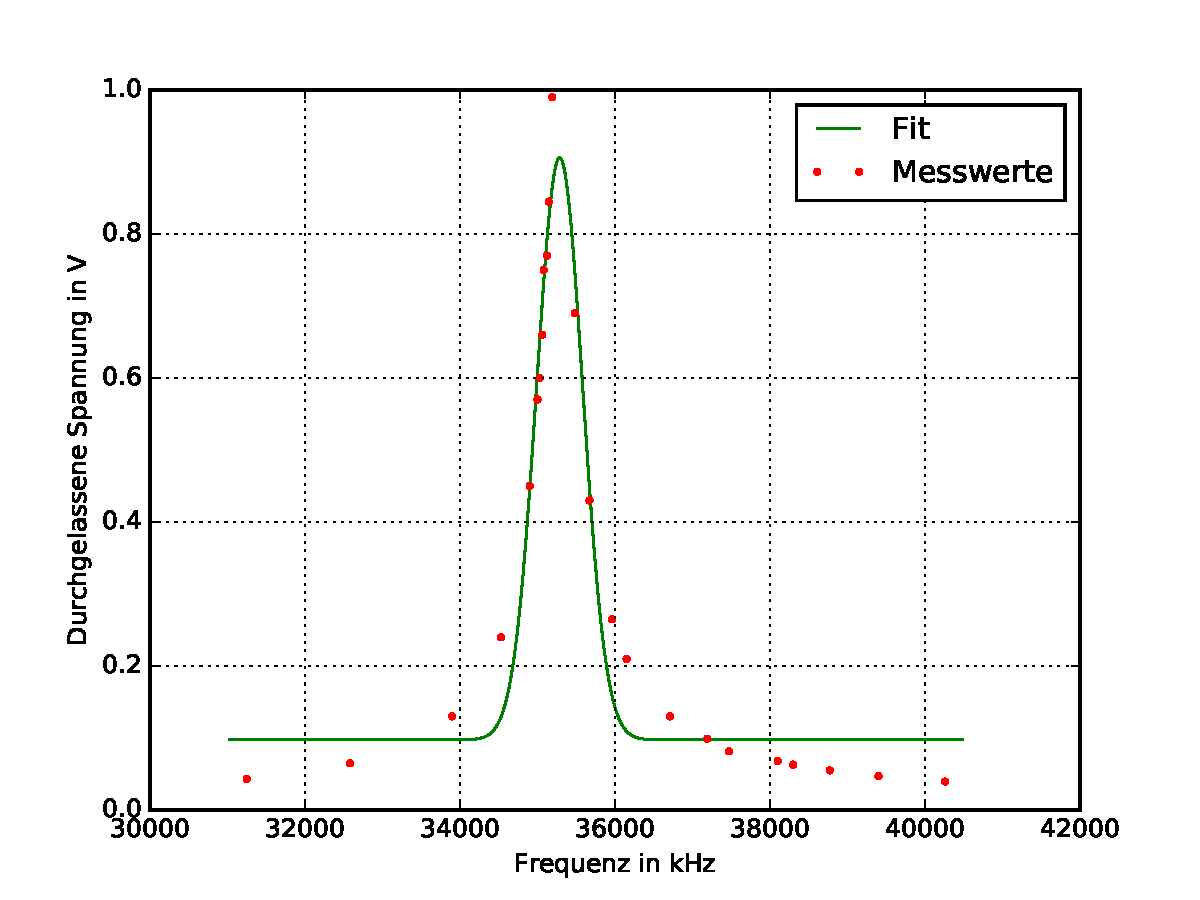
\includegraphics[width=\textwidth]{../plots/amplifier.pdf}
			\caption{Durchlasskurve des Selektiv-Verstärkers. Der Fit der Gaußkurve dient nur zum finden der Bandbreite; es reicht deswegen aus, dass dieser nur in der Nähe von $U = \nicefrac{1}{\sqrt{2}}\si{\V}$ genau ist.}
			\label{fig:_plots_amplifier_pdf_}
		\end{figure}

		Bei einer theoretischen Güte von 100 ist der Bandpass des Filters recht scharf. Die aus den Messdaten gewonnene Kurve hat eine Güte von

		\begin{align}\label{equ:guete}
			Q=\nicefrac{f_\text{Umax}}{f_\text{Bandbreite}} = 77.16 \;.
		\end{align}

		Das Spannungsmaximum von \SI{0.99}{\V} bei einer Speisespannung von etwa \SI{1}{\V} wird bei etwa \SI{35.19}{\k\Hz} eingenommen. Die Speisespannung bleibt in den folgenden Abschnitten gleich.
		Die Kurve wird ohne Verstärkung der Spannung aufgenommen.

	\subsection{Suszeptibilität}
	\label{sub:suszeptibilität}
		
		Die Suszeptibilität wird durch das Messen der Brückenspannung nach Stabeinführung ($\chi_U$) und das Vergleichen der Widerstände bei abgeglichener Brücke ($\chi_R$) bestimmt. Diese Werte weichen stark voneinander ab, der Mittelwert aus beiden liegt jedoch recht nahe an dem nach der Hund'schen Regel berechneten $\chi_\text{Hund}$.  
		Die Messungen werden mit einer um den Faktor 100 verstärkten Spannung durchgeführt.

		Die mithilfe der Hund'sche Regel bestimmten Parameter sind in Tabelle~\ref{tab:elektronenkonf} zu sehen; aus ihnen ergibt sich mit Gl.~\ref{equ:sub_calc} die Werte aus Tabelle~\ref{tab:results}. Es werden 15°C als Raumtemperatur angenommen.

		Zur besseren Einschätzung der Werte dient Abbildung~\ref{fig:_plots_chi_pdf}.

		\begin{table}[H]
		    \centering
		    \caption{Elektronenkonfiguration der 4f-Schale.}
		    \label{tab:elektronenkonf}
		    \begin{adjustbox}{center}
		    \begin{tabular}{
		        r
		        S
		        S
		        S}
		     \toprule
		     \multicolumn{1}{c}{} &
		     \multicolumn{1}{c}{$\text{Dy}^{3+}$} &
		     \multicolumn{1}{c}{$\text{Nd}^{3+}$} &
		     \multicolumn{1}{c}{$\text{Gd}^{3+}$} \\
		     \midrule
		     \primitiveinput{../tables/hund_params.tex}
		     \bottomrule
		    \end{tabular}
		    \end{adjustbox}
		\end{table}

		\begin{table}[H]
		    \centering
		    \caption{Messergebnisse beider Methoden und Vergleich mit der Hund'schen Regel. Die letzte Spalte bezeichnet die relative Abweichungen der verschiedenen Werte von den Vorhersagen nach Hund.}
		    \label{tab:results}
		    \begin{adjustbox}{center}
		    \begin{tabular}{
		    	r
		        r@{$\pm$}l
		        r@{$\pm$}l
		        c
		        c
		        c
		        c
		        c}
		     \toprule
		     \multicolumn{1}{c}{}&
		     \multicolumn{6}{c}{Suszeptibilitäten}&
		     \multicolumn{3}{c}{Abweichungen in \%}\\
		     \multicolumn{1}{c}{Ion} &
		     \multicolumn{2}{c}{$\chi_U$} &
		     \multicolumn{2}{c}{$\chi_R$} &
		     \multicolumn{1}{c}{$\chi_\text{mittel}$}&
		     \multicolumn{1}{c}{$\chi_\text{Hund}$}&
		     \multicolumn{1}{c}{$\chi_U$}&
		     \multicolumn{1}{c}{$\chi_R$}&
		     \multicolumn{1}{c}{$\chi_\text{mittel}$}\\
		     \midrule
		     \primitiveinput{../tables/chi-results.tex}
		     \bottomrule
		    \end{tabular}
		    \end{adjustbox}
		\end{table}

		\begin{figure}[H]
			\centering
			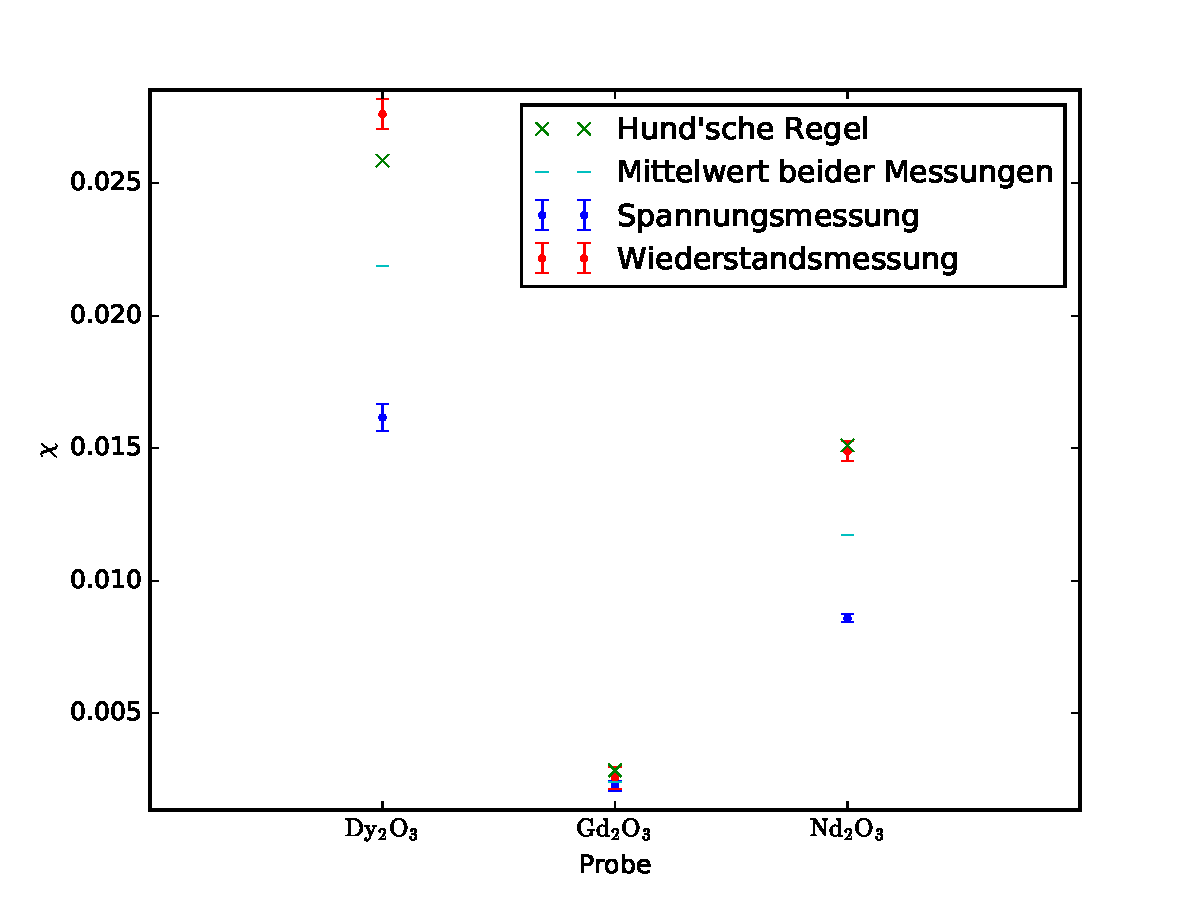
\includegraphics[width=\textwidth]{../plots/chi.pdf}
			\caption{Suszeptibilität der Proben im Vergleich.}
			\label{fig:_plots_chi_pdf}
		\end{figure}



	\subsection{Messdaten}
	\label{sub:messdaten}
		Da die Proben aus einem Pulver bestehen ist ihre Dichte geringer als die Dichte eines Einkristalls $\rho$. Mit der Masse $m$ der Probe und ihrer Länge $L$
		lässt sich der effektive Querschnitt $Q_\text{adj}$ berechnen:

			\begin{align*}
				Q_\text{adj} = \frac{m}{L \rho} \;.
			\end{align*}

		Die benutzte Spule hat einen Durchmesser von \SI{86.6}{10^{-6}\m^2}, die Brückenschaltung hat einen Nebenwiderstand von $R_3=\SI{998}{\ohm}$.
		Es folgt eine Auflistung der Messdaten und der daraus berechneten Zwischenergebnisse.

		\begin{table}[H]
		    \centering
		    \caption{Parameter der Proben.}
		    \label{tab:seern}
		    \begin{adjustbox}{center}
		    \begin{tabular}{
		    	l
		        S
		        S
		        S}
		     \toprule
		     \multicolumn{1}{c}{} &
		     \multicolumn{1}{c}{$\text{Dy}_2 \text{O}_3$} &
		     \multicolumn{1}{c}{$\text{Nd}_2 \text{O}_3$} &
		     \multicolumn{1}{c}{$\text{Gd}_2 \text{O}_3$} \\
		     \midrule
		     \primitiveinput{../tables/proben_parameter.tex}
		     \bottomrule
		    \end{tabular}
		    \end{adjustbox}
		\end{table}

		\begin{table}[H]
		    \centering
		    \caption{Messdaten zu Dy.}
		    \label{tab:mess_dy}
		    \begin{adjustbox}{center}
		    \begin{tabular}{
		        c
		        c
		        c
		        c}
		     \toprule
		     \multicolumn{1}{c}{$\chi_U$} &
		     \multicolumn{1}{c}{$U$ in \si{\nano \V}} &
		     \multicolumn{1}{c}{$\chi_R$} &
		     \multicolumn{1}{c}{$\Delta R$ in \si{\ohm}} \\
		     \midrule
		     \primitiveinput{../tables/data_element_0.tex}
		     \bottomrule
		    \end{tabular}
		    \end{adjustbox}
		\end{table}

		\begin{table}[H]
		    \centering
		    \caption{Messdaten zu Nd.}
		    \label{tab:mess_dy}
		    \begin{adjustbox}{center}
		    \begin{tabular}{
		        c
		        c
		        c
		        c}
		     \toprule
		     \multicolumn{1}{c}{$\chi_U$} &
		     \multicolumn{1}{c}{$U$ in \si{\nano \V}} &
		     \multicolumn{1}{c}{$\chi_R$} &
		     \multicolumn{1}{c}{$\Delta R$ in \si{\ohm}} \\
		     \midrule
		     \primitiveinput{../tables/data_element_1.tex}
		     \bottomrule
		    \end{tabular}
		    \end{adjustbox}
		\end{table}

		\begin{table}[H]
		    \centering
		    \caption{Messdaten zu Gd.}
		    \label{tab:mess_dy}
		    \begin{adjustbox}{center}
		    \begin{tabular}{
		        c
		        c
		        c
		        c}
		     \toprule
		     \multicolumn{1}{c}{$\chi_U$} &
		     \multicolumn{1}{c}{$U$ in \si{\nano \V}} &
		     \multicolumn{1}{c}{$\chi_R$} &
		     \multicolumn{1}{c}{$\Delta R$ in \si{\ohm}} \\
		     \midrule
		     \primitiveinput{../tables/data_element_2.tex}
		     \bottomrule
		    \end{tabular}
		    \end{adjustbox}
		\end{table}